\documentclass[12pt,a4paper]{article}
% Packages
\usepackage[utf8]{inputenc}
\usepackage[T1]{fontenc}
\usepackage{amsmath,amssymb}
\usepackage{graphicx}
\usepackage[hidelinks]{hyperref}
\usepackage{authblk} % Package for multiple authors
\usepackage{booktabs} % For better tables
\usepackage{listings} % For code snippets
\usepackage{xcolor} % For colored text
\usepackage{float} % For better figure placement with [H]
% Define Prolog language style for listings
\definecolor{prologcomment}{rgb}{0.5,0.5,0.5} % Gray for comments
\definecolor{prologkeyword}{rgb}{0,0,0.8} % Blue for keywords/predicates
\definecolor{prologstring}{rgb}{0.8,0,0} % Red for strings/atoms
\definecolor{prologvariable}{rgb}{0,0.5,0} % Green for variables
\lstdefinestyle{prologstyle}{
language=Prolog,
basicstyle=\ttfamily\small,
keywordstyle=\color{prologkeyword}\bfseries,
commentstyle=\color{prologcomment},
stringstyle=\color{prologstring},
identifierstyle=\color{prologvariable}, % Style for variables
morekeywords={node, arc, edge, find_simple_cycles, generate_edges_from_arcs, find_all_elementary_cycles, find_cycles_from_potential_starts, dfs_for_cycle, filter_to_simple_cycles, is_simple_cycle_candidate, check_all_node_pairs_for_chords, check_one_node_against_all_others, get_distance_along_cycle, find_shortest_path_length, bfs\_shortest_path, add_unvisited_neighbors_to_queue, normalize_cycle_representation, find_lexicographically_smallest_node, rotate_list_to_start_with_element, print_cycles_list, print_cycles_list_reversed, member, length, writeln, write, nl, retractall, forall, assertz, findall, reverse, append, nth0, list_to_set, setof, main, setup_test_graph, read, halt},
morecomment=[l]{//}, % Line comments starting with //
morecomment=[l]{\%}, % Line comments starting with %
morestring=[b]', % Single quoted strings/atoms
morestring=[b]", % Double quoted strings (less common in Prolog)
showstringspaces=false,
tabsize=2,
breaklines=true,
breakatwhitespace=true,
captionpos=b, % Position caption below the listing
frame=single % Add a frame around the code
}
% Title and author information
\title{Finding Simple Cycles in a Directed Graph using Prolog}
\author[1]{Cirilli Davide}
\author[2]{Fontana Emanuele}
\affil[1,2]{Department of Computer Science, Università degli Studi di Bari}
\begin{document}
\maketitle
\tableofcontents
\newpage
\section{Introduction}
A cycle in a directed graph is a path that starts and ends at the same node. An \textit{elementary cycle} is a cycle where no node (except the start/end node) appears more than once. This program aims to find a subset of elementary cycles termed "simple cycles".

A cycle is defined as \textit{simple} if, for any two distinct nodes 
$u$ 
 and 
$v$ 
 within the cycle, the shortest path from 
$u$ 
 to 
$v$ 
 in the \textit{entire graph} is the path that follows the edges of the cycle itself. If a shorter path (a "shortcut" or "chord") exists between 
$u$ 
 and 
$v$ 
 using edges outside the cycle, the cycle is not considered simple.

This document describes our Prolog program designed to identify all such "simple cycles" within a directed graph. The program features an interactive main predicate that allows selection from predefined test cases. For a chosen graph, it first finds all elementary cycles and then filters them based on the specific shortest path criterion described above to determine simplicity. The implementation utilizes Depth-First Search (DFS) for cycle detection and Breadth-First Search (BFS) for shortest path calculations.

This program implements this definition using Prolog, leveraging its backtracking capabilities for graph traversal and dynamic fact manipulation for setting up different graph structures.
\section{Implementation Details}
The Prolog program (\texttt{simpleCycle.pl}) begins with directives:
\begin{verbatim}
:- dynamic node/2.
:- dynamic arc/4.
:- dynamic edge/2.
\end{verbatim}
The \texttt{:- dynamic Predicate/Arity} directive declares that facts for \texttt{node/2}, \texttt{arc/4}, and the helper \texttt{edge/2} can be added (\texttt{assertz}) or removed (\texttt{retractall}) during program execution. This is crucial for the \texttt{setup\_test\_graph/1} predicate, which defines different graph structures, and for \texttt{generate\_edges\_from\_arcs/0}, which dynamically creates \texttt{edge/2} facts.
The program consists of several key components:
\subsection{Graph Representation and Setup}
The graph is primarily defined by \texttt{arc/4} facts, which are dynamically asserted by test case setup predicates.
\begin{itemize}
\item \texttt{node(NodeID, Type)}: Declares a node with a unique ID and an associated type. While test cases primarily define connectivity through \texttt{arc/4} facts, default \texttt{node/2} facts are provided in the code. These are used by \texttt{find\_all\_elementary\_cycles/1} to gather an initial list of all potential starting nodes for cycle detection.
\item \texttt{arc(ArcID, Type, SourceNode, TargetNode)}: Declares an arc with a unique ID, type, source node, and target node. These facts define the graph's structure for a given test case.
\item \texttt{setup\_test\_graph/1}: A predicate responsible for configuring the graph for a chosen test case (1, 2, 3, or 4). It first calls \texttt{retractall(arc(\_, \_, \_, \_))} to clear any existing arc definitions and then asserts the specific \texttt{arc/4} facts for the selected test case.
\end{itemize}
For traversal efficiency, a helper predicate \texttt{edge(Source, TargetNode)} is dynamically generated from the current \texttt{arc/4} facts.
\begin{itemize}
\item \texttt{generate\_edges\_from\_arcs/0}: This predicate prepares the graph for traversal.
\begin{itemize}
\item It first calls \texttt{retractall(edge(\_, \_))} to remove any existing \texttt{edge/2} facts, ensuring a clean state corresponding to the current set of \texttt{arc/4} facts.
\item Then, \texttt{forall(arc(\_, \_, SourceNode, DestinationNode), assertz(edge(SourceNode, DestinationNode)))} iterates through all current \texttt{arc/4} facts. For each, it extracts the source (\texttt{SourceNode}) and target (\texttt{DestinationNode}) nodes and asserts a new fact \texttt{edge(SourceNode, DestinationNode)}. This provides faster lookups for direct connections.
\end{itemize}
\end{itemize}
\subsection{Finding Elementary Cycles}
Elementary cycles are found using a Depth-First Search (DFS) approach:
\begin{itemize}
\item \texttt{find\_all\_elementary\_cycles/1}: The main predicate for this stage.
\begin{itemize}
\item It uses \texttt{findall(NodeID, node(NodeID, \_NodeType), Nodes)} to collect all \texttt{NodeID}s from the currently asserted \texttt{node/2} facts into the list \texttt{Nodes}. These nodes serve as potential starting points for cycles.
\item It then calls \texttt{find\_cycles\_from\_potential\_starts/2} with this list.
\item The argument \texttt{ElementaryCyclesList} will be unified with the list of all elementary cycles found.
\end{itemize}
\item \texttt{find\_cycles\_from\_potential\_starts/2}: Iterates through all nodes from the \texttt{Nodes} list and initiates DFS from each.
\begin{itemize}
\item It uses \texttt{findall/3}. The template is \texttt{RawCycle}.
\item The goal is \texttt{(member(StartNode, PotentialStartNodes), edge(StartNode, FirstNeighbor), dfs\_for\_cycle(FirstNeighbor, StartNode, [FirstNeighbor, StartNode], RawCycle))}.
\item \texttt{member(StartNode, PotentialStartNodes)} iterates through each node as a potential starting point.
\item \texttt{edge(StartNode, FirstNeighbor)} finds a node directly reachable from \texttt{StartNode}.
\item \texttt{dfs\_for\_cycle/4} is called to perform DFS starting from this \texttt{Neighbor}, aiming to return to \texttt{StartNode}. The path is initialized with \texttt{[Neighbor, StartNode]}.
\item \texttt{findall/3} collects all \texttt{RawCycle} bindings found through backtracking.
\end{itemize}
\item \texttt{dfs\_for\_cycle/4}: Performs the recursive DFS: \texttt{dfs\_for\_cycle(CurrentNode, TargetNode, PathBackToStart, FoundCycleInReverse)}.
\begin{itemize}
\item It looks for an edge from \texttt{CurrentNode} to \texttt{NextNode} using \texttt{edge(CurrentNode, NextNode)}.
\item Base Case: If \texttt{NextNode == TargetNode}, the starting node is reached. \texttt{FoundCycleInReverse} is unified with \texttt{[TargetNode | PathBackToStart]}.
\item Recursive Step: If \texttt{NextNode} is not \texttt{TargetNode}, it checks \texttt{\textbackslash+ memberchk(NextNode, PathBackToStart)} to ensure elementarity. If not visited in the current path, it recursively calls \texttt{dfs\_for\_cycle(NextNode, TargetNode, [NextNode | PathBackToStart], FoundCycleInReverse)}.
\end{itemize}
\item Cycles from DFS are returned in reverse traversal order (e.g., \texttt{[a, d, c, b, a]} for a cycle $a \rightarrow b \rightarrow c \rightarrow d \rightarrow a$). 
\end{itemize}
\subsection{Filtering for Simple Cycles}
The logic for identifying simple cycles:
\begin{itemize}
\item \texttt{filter\_to\_simple\_cycles/2}: Takes \texttt{ElementaryCyclesRaw} and returns \texttt{NormalizedSimpleCyclesCandidates}.
\begin{itemize}
\item Base Case: \texttt{filter\_to\_simple\_cycles([], [])}.
\item Recursive Step 1 (Simple Cycle Found): If \texttt{is\_simple\_cycle\_candidate(CandidateCycle)} succeeds for the head \texttt{Cycle}, it's cut (\texttt{!}), normalized via \texttt{normalize\_cycle\_representation\_representation(CandidateCycle, NormalizedCycle)}, and prepended to the result of recursively processing \texttt{RestCandidates}.
\item Recursive Step 2 (Not Simple): If \texttt{is\_simple\_cycle\_candidate(CandidateCycle)} fails, the \texttt{\_Cycle} is ignored, and the predicate recurses on \texttt{RestCandidates}.
\end{itemize}
\item \texttt{is\_simple\_cycle\_candidate/1}: Checks if an elementary cycle is simple.
\begin{itemize}
\item Reverses the DFS cycle: \texttt{reverse(ReversedCycleFromDFS, ForwardCycleWithRepeatEnd)}.
\item Deconstructs to get ordered unique nodes: \texttt{ForwardCycleWithRepeatEnd = [StartNode | PathNodesWithRepeatEnd]}, \texttt{append(PathNodesUnique, [StartNode], PathNodesWithRepeatEnd)}, \texttt{NodesInCycleOrdered = [StartNode | PathNodesUnique]}. E.g., for DFS output \texttt{[a,c,b,a]}, this yields \texttt{[a,b,c]}.
\item Calls \texttt{check\_all\_node\_pairs\_for\_chords(CycleNodesInOrder, CycleNodesInOrder)}.
\end{itemize}
\item \texttt{check\_all\_node\_pairs\_for\_chords/2}: Iterates through ordered pairs $(u,v)$ 
 in \texttt{CycleNodesInOrder}.
\begin{itemize}
\item Base Case: \texttt{check\_all\_node\_pairs\_for\_chords([], \_)}.
\item Recursive Step: Takes \texttt{Node1} from the list, calls \newline \texttt{check\_one\_node\_against\_all\_others(Node1, OriginalCycleNodesOrdered, OriginalCycleNodesOrdered)}, then recurses on \texttt{RestN1}.
\end{itemize}
\item \texttt{check\_one\_node\_against\_all\_others/3}: For a given \texttt{Node1}, iterates through other nodes \texttt{Node2} in \texttt{OriginalCycleNodesOrdered}.
\begin{itemize}
\item Base Case: \texttt{check\_one\_node\_against\_all\_others(\_, [], \_)}.
\item Recursive Step: Takes \texttt{Node2}.
\item If \texttt{Node1 == Node2}, skip (\texttt{true}).
\item Else, calculate \texttt{get\_distance\_along\_cycle(Node1, Node2, OriginalCycleNodesOrdered, CycleDist)} and \texttt{find\_shortest\_path\_length(Node1, Node2, GraphShortestDistance)}.
\item Check simplicity:
\begin{itemize}
\item If \texttt{GraphShortestDistance == -1} (no path in graph), then $CycleDist > 0$ 
 must hold (or \texttt{!, fail}).
\item Else (path exists), $GraphShortestDistance \ge CycleDist$ 
 must hold.
\end{itemize}
\item If the check succeeds, cut (\texttt{!}) and recurse on \texttt{RestN2}.
\item Failure Clause: \texttt{check\_one\_node\_against\_all\_others(\_, \_, \_) :- !, fail.} ensures immediate failure if any pair violates simplicity.
\end{itemize}
\item \texttt{get\_distance\_along\_cycle/4}: Calculates distance from \texttt{NodeA} to \texttt{NodeB} along \texttt{CycleNodesOrdered}.
\begin{itemize}
\item Finds indices \texttt{IndexA}, \texttt{IndexB} using \texttt{nth0/3}. Gets \texttt{length(CycleNodesOrdered, PathLength)}.
\item If $IndexB \ge IndexA$, $Distance = IndexB - IndexA$. 
\item Else, $Distance = PathLength - IndexA + IndexB$. 
\end{itemize}
\item \texttt{find\_shortest\_path\_length/3}: Finds shortest path length between \texttt{StartNode} and \texttt{EndNode} using BFS.
\begin{itemize}
\item Calls \texttt{bfs\_shortest\_path([[StartNode, 0]], EndNode, [StartNode], Length)}.
\item Cuts (\texttt{!}) on success. If BFS fails, the second clause \texttt{find\_shortest\_path\_length(\_, \_, -1)} sets \texttt{Length} to -1.
\end{itemize}
\item \texttt{bfs\_shortest\_path/4}: Standard BFS: \texttt{bfs\_shortest\_path(Queue, TargetNode, VisitedNodes, PathLength)}.
\begin{itemize}
\item Base Case 1 (Queue Empty): \texttt{bfs\_shortest\_path([], \_, \_, \_) :- !, fail.}
\item Base Case 2 (TargetNode Found): \texttt{bfs\_shortest\_path([[TargetNode, PathLength] | \_], TargetNode, \_, PathLength) :- !.}
\item Recursive Step: Dequeues \texttt{[CurrentNode, CurrentDist]}. Finds unvisited neighbors via \texttt{findall(NextNode, (edge(CurrentNode, NextNode), \textbackslash+ member(NextNode, VisitedNodes)), UnvisitedNeighbors)}. Calculates $NewDistToNeighbors = CurrentDist + 1$. 
 Adds neighbors to queue via \texttt{add\_unvisited\_neighbors\_to\_queue/4}. Updates visited list (using \texttt{append/3} and \texttt{list\_to\_set/2}). Recurses.
\end{itemize}
\item \texttt{add\_unvisited\_neighbors\_to\_queue/4}: Formats neighbors as \texttt{[Node, Distance]} and appends to queue using \texttt{findall/3} and \texttt{append/3}.
\end{itemize}
\subsection{Cycle Normalization}
Ensures unique representation for identical cycles starting at different nodes.
\begin{itemize}
\item \texttt{normalize\_cycle\_representation/2}: Converts raw DFS cycle \texttt{RawReversedCycle} (e.g., \texttt{[a,d,c,b,a]}) to \texttt{NormalizedNodeList}.
\item Process:
\begin{enumerate}
\item Deconstruct: \texttt{RawReversedCycle = [StartNode | PathReversedWithStartNodeAtEnd]}.
\item Get forward path nodes: \texttt{reverse(PathReversedWithStartNodeAtEnd, [\_StartNodeAgain | PathForwardWithoutStartNode])}.
\item Reconstruct forward cycle nodes: \texttt{CycleNodesInForwardOrder = [StartNode | PathForwardWithoutStartNode]} (e.g., \texttt{[a,b,c,d]}).
\item Find minimum node: \texttt{find\_lexicographically\_smallest\_node(CycleNodesInForwardOrder, SmallestNode)}.
\item Rotate: \texttt{rotate\_list\_to\_start\_with\_element(CycleNodesInForwardOrder, SmallestNode, NormalizedNodeList)}.
\end{enumerate}
\item \texttt{find\_lexicographically\_smallest\_node/2}: Finds minimum node in a list using \texttt{@<}.
\begin{itemize}
\item Base Case: \texttt{find\_lexicographically\_smallest\_node([Min], Min) :- !.}
\item Recursive Step: Compares head \texttt{Head} with minimum of tail \texttt{MinOfTail}.
\end{itemize}
\item \texttt{rotate\_list\_to\_start\_with\_element/3}: Rotates \texttt{OriginalList} so \texttt{StartElement} is first.
\begin{itemize}
\item Uses \texttt{append(BeforeElement, [StartElement | AfterElement], OriginalList), !, append([StartElement | AfterElement], BeforeElement, RotatedList)}.
\item Fallback clause: \texttt{rotate\_list\_to\_start\_with\_element(OriginalList, \_, OriginalList)} if element already first or not found (latter shouldn't occur in this program's logic).
\end{itemize}
\end{itemize}
The final list of simple cycles is produced using \texttt{setof/3} on the normalized cycles to ensure uniqueness and canonical order.
\subsection{Main Predicate and Output Control}
\begin{itemize}
\item \texttt{main/0}: The primary entry point for execution.
\begin{enumerate}
\item Prompts the user to select a test case (1-4) using \texttt{write/1} and \texttt{read/1}.
\item Calls \texttt{setup\_test\_graph(testCaseNumber)} with the chosen number \texttt{N}.
\item If \texttt{setup\_test\_graph\_graph/1} succeeds, it calls \texttt{find\_simple\_cycles(SimpleCyclesList)}.
\item Prints the resulting \texttt{SimpleCyclesList} list.
\item If an invalid test case number is entered, an error message is shown.
\item Calls \texttt{halt/0} to terminate the Prolog session.
\end{enumerate}
\item \texttt{find\_simple\_cycles/1}: Orchestrates the cycle finding and filtering process for the currently loaded graph.
\begin{enumerate}
\item Calls \texttt{generate\_edges\_from\_arcs/0}.
\item Calls \texttt{find\_all\_elementary\_cycles/1} to get \texttt{ElementaryCyclesRaw}.
\item Prints the count and list of elementary cycles (using \texttt{print\_cycles\_list\_reversed/2} as DFS cycles are reversed).
\item If elementary cycles exist:
\begin{itemize}
\item Calls \texttt{filter\_to\_simple\_cycles/2} to get \texttt{NormalizedSimpleCyclesCandidates}.
\item Uses \texttt{setof(NormCycle, Member\textasciicircum{}(member(Member, NormalizedSimpleCyclesCandidates), NormCycle = Member), SimpleCyclesList)} to get the final unique, sorted list.
\item Prints the simple cycles (using \texttt{print\_cycles\_list/2}) and their count.
\item If \texttt{setof/3} fails (no simple cycles), prints a message and sets \texttt{SimpleCyclesList} to \texttt{[]}.
\end{itemize}
\item If no elementary cycles, prints a message and sets \texttt{SimpleCyclesList} to \texttt{[]}.
\item The argument \texttt{SimpleCyclesList} is unified with the final list.
\end{enumerate}
\item Helper Printing Predicates:
\begin{itemize}
\item \texttt{print\_cycles\_list/2}: \texttt{print\_cycles\_list(Header, ListOfCycles)}. Prints a header and then each cycle in the list, indented.
\item \texttt{print\_cycles\_list\_reversed/2}: Similar to \texttt{print\_cycles\_list/2}, but it first reverses each cycle in the list before printing. This is used for displaying elementary cycles as found by DFS in their natural traversal order.
\end{itemize}
\end{itemize}
\section{Test Cases and Usage}
\subsection{Usage}
Ensure a Prolog interpreter (e.g., SWI-Prolog) is installed.
Load the program file: \texttt{?- [simpleCycle].} (or your filename).
Run the main interactive predicate: \texttt{?- main.}
The program will prompt: \texttt{Select test case (1, 2, 3, or 4):}
Enter a number from 1 to 4 and press Enter.
The program will then execute for the chosen test case, printing intermediate elementary cycles and the final list of unique, normalized simple cycles. The output will also show \texttt{SimpleCycles = [[...], ...]}.
The program will then halt.
\subsection{Predefined Test Cases}
The program includes four predefined test cases, set up by \texttt{setup\_test\_graph/1}.
\subsubsection{Test Case 1: Simple Triangle}
\begin{itemize}
\item \textbf{Description:} A basic directed triangle: $a \rightarrow b \rightarrow c \rightarrow a$. 
\item \textbf{Arcs Defined:}
\begin{lstlisting}[style=prologstyle, basicstyle=\ttfamily\footnotesize]
assertz(arc(t1_ab, type_edge, a, b)).
assertz(arc(t1_bc, type_edge, b, c)).
assertz(arc(t1_ca, type_edge, c, a)).
\end{lstlisting}
\item \textbf{Graph Visualization:}
\begin{figure}[H]
\centering
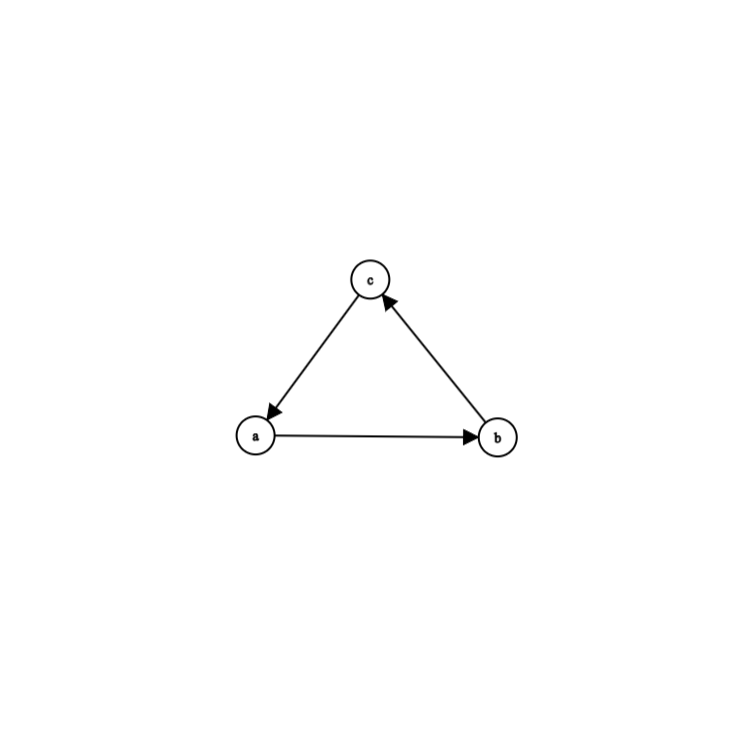
\includegraphics[width=0.7\textwidth]{img/Test1.png} % Replace with actual image path
\caption{Graphical representation of Test Case 1.}
\label{fig:testcase1}
\end{figure}
\item \textbf{Expected Simple Cycles:} \texttt{[[a,b,c]]}
\end{itemize}
\subsubsection{Test Case 2: Square with a Chord}
\begin{itemize}
\item \textbf{Description:} A square cycle $a \rightarrow b \rightarrow c \rightarrow d \rightarrow a$, with an additional "chord" arc $b \rightarrow d$. 
\item \textbf{Arcs Defined:}
\begin{lstlisting}[style=prologstyle, basicstyle=\ttfamily\footnotesize]
assertz(arc(t2_ab, type_edge, a, b)).
assertz(arc(t2_bc, type_edge, b, c)).
assertz(arc(t2_cd, type_edge, c, d)).
assertz(arc(t2_da, type_edge, d, a)).
assertz(arc(t2_bd_chord, type_edge, b, d)). % The chord
\end{lstlisting}
\item \textbf{Graph Visualization:}
\begin{figure}[H]
\centering
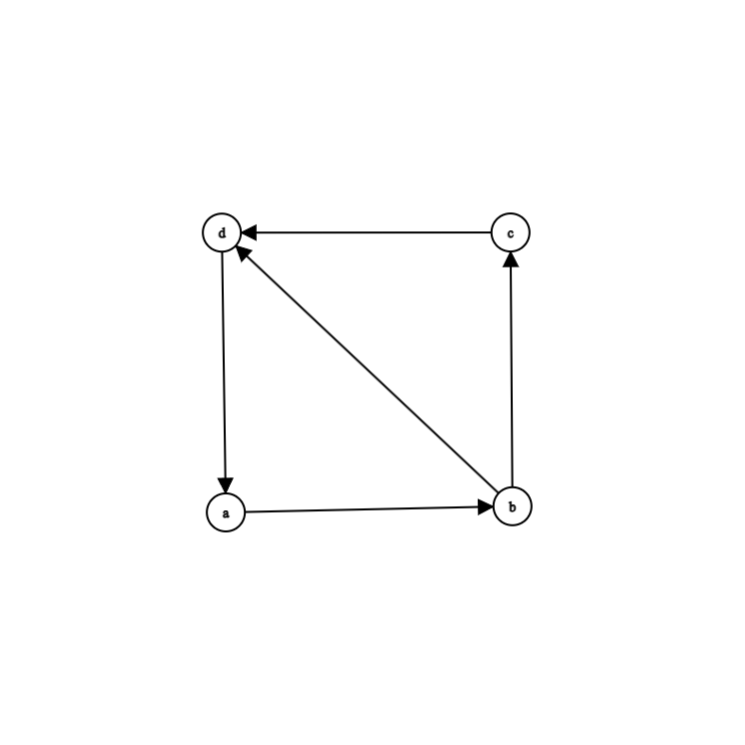
\includegraphics[width=0.7\textwidth]{img/Test2.png} % Replace with actual image path
\caption{Graphical representation of Test Case 2.}
\label{fig:testcase2}
\end{figure}
\item \textbf{Expected Simple Cycles:} \texttt{[[a,b,d], [b,c,d]]}. The cycle \texttt{[a,b,c,d]} (from $a \rightarrow b \rightarrow c \rightarrow d \rightarrow a$) is elementary but not simple due to the shortcut $b \rightarrow d$ (path $b \rightarrow c \rightarrow d$ has length 2, path $b \rightarrow d$ has length 1). 
\end{itemize}
\subsubsection{Test Case 3: Disjoint Cycles}
\begin{itemize}
\item \textbf{Description:} A graph containing a 2-cycle ($a \leftrightarrow b$) and two separate, non-overlapping triangles ($c \rightarrow d \rightarrow e \rightarrow c$ and $d \rightarrow f \rightarrow g \rightarrow d$). 
\item \textbf{Arcs Defined:}
\begin{lstlisting}[style=prologstyle, basicstyle=\ttfamily\footnotesize]
assertz(arc(t3_ab, type_edge, a, b)). % 2-cycle
assertz(arc(t3_ba, type_edge, b, a)).
assertz(arc(t3_cd, type_edge, c, d)). % Triangle 1
assertz(arc(t3_de, type_edge, d, e)).
assertz(arc(t3_ec, type_edge, e, c)).
assertz(arc(t3_df, type_edge, d, f)). % Triangle 2
assertz(arc(t3_fg, type_edge, f, g)).
assertz(arc(t3_gd, type_edge, g, d)).
\end{lstlisting}
\item \textbf{Graph Visualization:}
\begin{figure}[H]
\centering
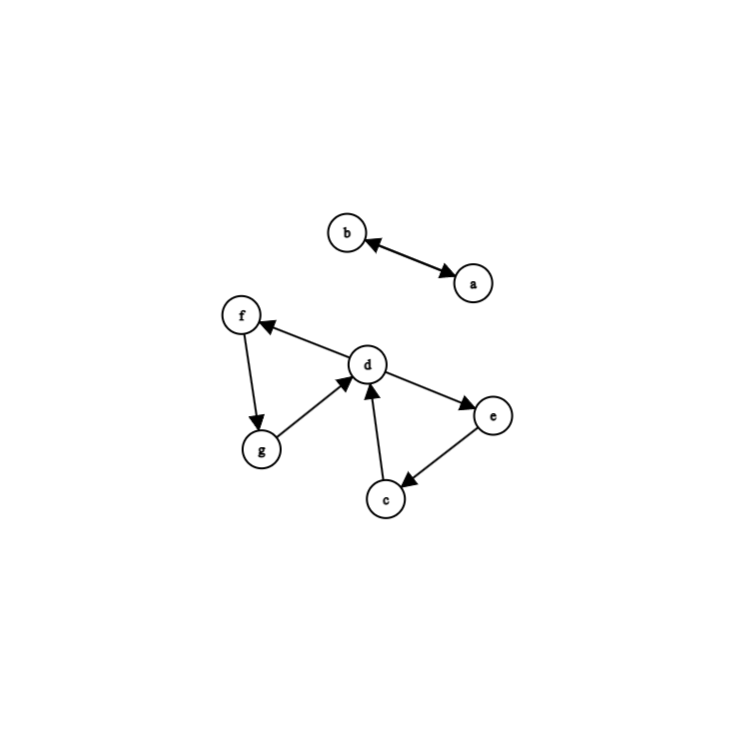
\includegraphics[width=0.7\textwidth]{img/Test3.png} % Replace with actual image path
\caption{Graphical representation of Test Case 3.}
\label{fig:testcase3}
\end{figure}
\item \textbf{Expected Simple Cycles:} \texttt{[[a,b], [c,d,e], [d,f,g]]} (order by \texttt{setof} might vary but content is these three).
\end{itemize}
\subsubsection{Test Case 4: Complex Overlapping Cycles and Chord}
\begin{itemize}
\item \textbf{Description:} A more complex graph with two larger, overlapping cycles and a shortcut arc.
Cycle A: $a \rightarrow b \rightarrow c \rightarrow d \rightarrow a$. 
Cycle B: $b \rightarrow e \rightarrow d \rightarrow c \rightarrow b$. 
Chord: $a \rightarrow d$. 
This also creates smaller 2-cycles like $b \leftrightarrow c$ and $c \leftrightarrow d$ due to edges from both Cycle A and Cycle B. 
\item \textbf{Arcs Defined:}
\begin{lstlisting}[style=prologstyle, basicstyle=\ttfamily\footnotesize]
assertz(arc(t4_ab, type_edge, a, b)).
assertz(arc(t4_bc, type_edge, b, c)).
assertz(arc(t4_cd, type_edge, c, d)).
assertz(arc(t4_da, type_edge, d, a)).
assertz(arc(t4_be, type_edge, b, e)).
assertz(arc(t4_ed, type_edge, e, d)).
assertz(arc(t4_dc, type_edge, d, c)). % Edge for Cycle B, opposite of c->d in Cycle A
assertz(arc(t4_cb, type_edge, c, b)). % Edge for Cycle B, opposite of b->c in Cycle A
assertz(arc(t4_ad_chord, type_edge, a, d)). % Chord for Cycle A
\end{lstlisting}
\item \textbf{Graph Visualization:}
\begin{figure}[H]
\centering
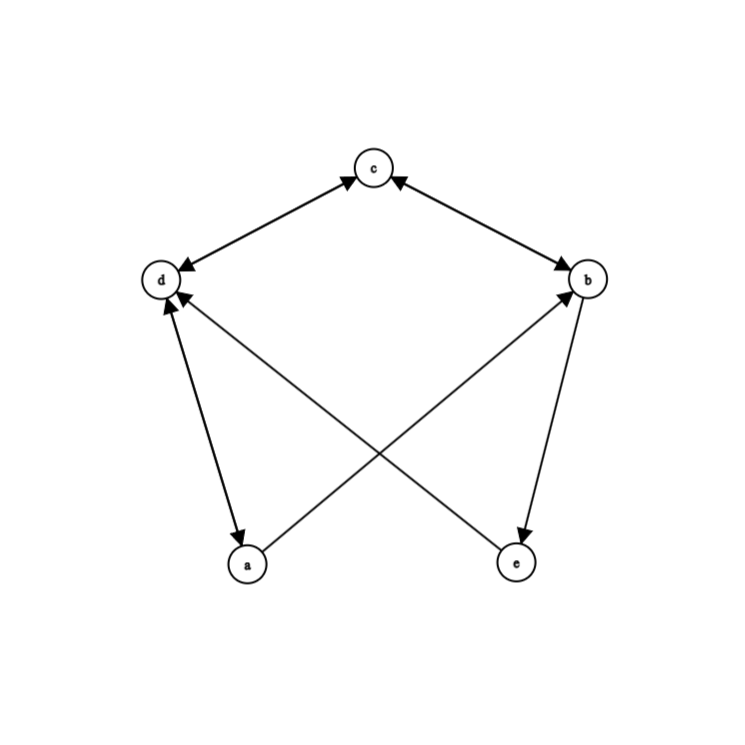
\includegraphics[width=0.7\textwidth]{img/Test4.png} % Replace with actual image path
\caption{Graphical representation of Test Case 4.}
\label{fig:testcase4}
\end{figure}
\item \textbf{Expected Simple Cycles:} \texttt{[[a,d], [b,c], [c,d]]}.
\begin{itemize}
\item \texttt{[a,b,c,d]} (from $a \rightarrow b \rightarrow c \rightarrow d \rightarrow a$) is not simple because path $a \rightarrow b \rightarrow c \rightarrow d$ (length 3) is longer than direct shortcut $a \rightarrow d$ (length 1). 
\item \texttt{[b,e,d,c]} (from $b \rightarrow e \rightarrow d \rightarrow c \rightarrow b$) is not simple because path $b \rightarrow e \rightarrow d \rightarrow c$ (length 3) is longer than direct shortcut $b \rightarrow c$ (length 1, via arc 2). 
\item The 2-cycles \texttt{[a,d]} ($a \rightarrow d$, $d \rightarrow a$), \texttt{[b,c]} ($b \rightarrow c$, $c \rightarrow b$), and \texttt{[c,d]} ($c \rightarrow d$, $d \rightarrow c$) are simple as their constituent 1-edge paths are inherently the shortest. 
\end{itemize}
\end{itemize}

\section{Implementation for Undirected Graphs}

In addition to the algorithm for directed graphs described in the previous sections, a variant for undirected graphs has been developed in the file \texttt{simpleCycleUndirected.pl}. The main differences between the two implementations are described below:

\subsection{Edge Generation in Undirected Graphs}
The main difference in the implementation for undirected graphs lies in the generation of \texttt{edge/2} facts from the arcs defined via \texttt{arc/4}:

\begin{itemize}
\item \texttt{generate\_edges\_from\_arcs/0}: While in the directed version each arc \texttt{arc(ID, Type, Source, Destination)} generates a single fact \texttt{edge(Source, Destination)}, in the undirected version each arc generates two facts: \texttt{edge(Source, Destination)} and \texttt{edge(Destination, Source)}, ensuring duplicates are avoided:

\begin{lstlisting}[style=prologstyle, basicstyle=\ttfamily\footnotesize]
generate_edges_from_arcs :-
    retractall(edge(_, _)),
    forall(arc(_ArcID, _ArcType, SourceNode, DestinationNode),
           (   (   \+ edge(SourceNode, DestinationNode)
               ->  assertz(edge(SourceNode, DestinationNode))
               ;   true
               ),
               (   \+ edge(DestinationNode, SourceNode)
               ->  assertz(edge(DestinationNode, SourceNode))
               ;   true
               )
           )).
\end{lstlisting}
\end{itemize}

\subsection{Finding Elementary Cycles in Undirected Graphs}
The DFS procedure has been modified to avoid spurious cycles that can arise from immediately returning to the previous node in an undirected graph:

\begin{itemize}
\item \texttt{dfs\_for\_cycle/4}: In the version for undirected graphs, the predicate keeps track of the immediate predecessor in the path and ensures that the next node to visit is not this predecessor:

\begin{lstlisting}[style=prologstyle, basicstyle=\ttfamily\footnotesize]
dfs_for_cycle(CurrentNode, TargetNode, PathBackToStart, FoundCycleInReverse) :-
    PathBackToStart = [CurrentNode, Prev | _],  % Extracts the immediate predecessor
    edge(CurrentNode, NextNode),                % Explores an edge from CurrentNode to NextNode
    (   % If NextNode is the target and not the immediate predecessor, a cycle is found
        NextNode == TargetNode,
        NextNode \== Prev
    ->  FoundCycleInReverse = [TargetNode | PathBackToStart]
    ;   % Otherwise, if NextNode is not the target, ensure it's not the immediate predecessor
        NextNode \== Prev,
        \+ memberchk(NextNode, PathBackToStart)  % Ensures NextNode is not already in the path
    ->  dfs_for_cycle(NextNode, TargetNode, [NextNode | PathBackToStart], FoundCycleInReverse)
    ).
\end{lstlisting}

This contrasts with the version for directed graphs, where it is not necessary to explicitly exclude the predecessor, because if an arc exists from $A$ to $B$, an arc from $B$ to $A$ does not necessarily exist:

\begin{lstlisting}[style=prologstyle, basicstyle=\ttfamily\footnotesize]
dfs_for_cycle(CurrentNode, TargetNode, PathBackToStart, FoundCycleInReverse) :-
    edge(CurrentNode, NextNode),
    (   NextNode == TargetNode ->
        FoundCycleInReverse = [TargetNode | PathBackToStart]
    ;   \+ memberchk(NextNode, PathBackToStart),
        dfs_for_cycle(NextNode, TargetNode, [NextNode | PathBackToStart], FoundCycleInReverse)
    ).
\end{lstlisting}
\end{itemize}

\subsection{Chord Detection in Undirected Graphs}
The version for undirected graphs must handle chord checking in a particular way to avoid false positives:

\begin{itemize}
\item \texttt{check\_one\_node\_against\_all\_others/3}: In the undirected version, the check skips pairs of adjacent nodes in the cycle (in both directions) to avoid confusing the cycle's own edges with possible chords:

\begin{lstlisting}[style=prologstyle, basicstyle=\ttfamily\footnotesize]
check_one_node_against_all_others(Node1, [Node2 | Rest], CycleNodesOrdered) :-
    (   Node1 == Node2
    ;   (get_distance_along_cycle(Node1, Node2, CycleNodesOrdered, D1), D1 =:= 1)
    ;   (get_distance_along_cycle(Node2, Node1, CycleNodesOrdered, D2), D2 =:= 1)
    )
    ->  true  % trivial: same node or adjacent in the undirected cycle
    ;   % Not adjacent: ensure no shorter path exists in the graph (no chords)
        get_distance_along_cycle(Node1, Node2, CycleNodesOrdered, CyclePathDistance),
        find_shortest_path_length(Node1, Node2, GraphShortestDistance),
        (   GraphShortestDistance == -1
        ->  CyclePathDistance > 0  % disconnected outside the cycle
        ;   GraphShortestDistance >= CyclePathDistance
        )
    ,
    !,
    check_one_node_against_all_others(Node1, Rest, CycleNodesOrdered).
\end{lstlisting}
\end{itemize}

\subsection{Cycle Normalization for Undirected Graphs}
A cycle in an undirected graph can be traversed in both directions. The undirected version normalizes cycles by considering both possible directions:

\begin{itemize}
\item \texttt{normalize\_cycle\_representation\_representation/2}: Generates two canonical representations (one for each traversal direction) and chooses the lexicographically smaller one as the canonical representation:

\begin{lstlisting}[style=prologstyle, basicstyle=\ttfamily\footnotesize]
normalize_cycle_representation_representation(RawReversedCycle, NormalizedNodeList) :-
    % Step 1: Convert DFS output to an ordered list of unique nodes (CycleForward)
    RawReversedCycle = [StartNode | PathRevEnd],
    reverse(PathRevEnd, [_StartAgain | PathForwardREST]),
    CycleForward = [StartNode | PathForwardREST],

    % Step 2: Normalize CycleForward starting from the lexicographically smallest node
    find_lexicographically_smallest_node(CycleForward, SmallestF),
    rotate_list_to_start_with_element(CycleForward, SmallestF, RotFwd),

    % Step 3: Generate and normalize the cycle in the opposite direction
    reverse(CycleForward, CycleBackwardTemp),
    find_lexicographically_smallest_node(CycleBackwardTemp, SmallestB),
    rotate_list_to_start_with_element(CycleBackwardTemp, SmallestB, RotBwd),

    % Step 4: Choose the lexicographically smaller list as the canonical representation
    (  RotFwd @=< RotBwd
    -> NormalizedNodeList = RotFwd
    ;  NormalizedNodeList = RotBwd
    ).
\end{lstlisting}
\end{itemize}

This improved normalization ensures that equivalent cycles (traversed in different directions) are represented consistently, facilitating the identification of unique cycles in undirected graphs.

\section{Conclusion}
The Prolog program successfully implements an algorithm to find simple cycles in both directed and undirected graphs, using the approach described in the previous sections. The version for undirected graphs (\texttt{simpleCycleUndirected.pl}) extends the base implementation (\texttt{simpleCycle.pl}) with specialized modifications to handle the bidirectionality of edges. Both implementations demonstrate the effective use of DFS for cycle detection, BFS for calculating shortest paths, and Prolog's capabilities for dynamic fact and list manipulation. Cycle normalization ensures that equivalent cycles are represented consistently, and \texttt{setof/3} provides a final, ordered list of these unique simple cycles.
\end{document}